\graphicspath{{./Paper5/}}

\begin{abstract}
The introduction of graphics processing unit (GPU) computing has made it possible to speed up computationally demanding algorithms. One of these algorithms is the calculation of pressure fields from acoustic transducers. Here, the execution time often limits the number of elements and field points we can select in order to get results back in finite time. 

In this paper we present a simple GPU-based simulator capable of simulating high resolution pressure fields at interactive frame rates. The simulator is based on the same principle as the Ultrasim toolbox, where responses from several point sources are accumulated in a set of observation points, hence solving the Rayleigh-Sommerfeld integral. The cumulative sum for each observation point is independent of all other observation points, making the problem perfect for GPU processing. For the simulator we provide both a Paint-like interface for interactive drawing of uniform linear arrays and free-hand shapes, and a Matlab interface for precise scripting of element positions and observation points.

The presented GPU simulator was compared both with a multi threaded C-version, Ultrasim, and Field II. Compared with Ultrasim we report a 400 times speedup when simulating a varying number of source points on a 150 K points observation grid. The test system consisted of a low-end GPU (Nvidia Quadro 600) and an Intel i7-870 2.93 GHz quad-core CPU.

\end{abstract}

\section{Introduction}
Software for simulation of pressure fields from ultrasound transducers is an important tool for gaining knowledge on how a transducer performs. This brings both great insight to researchers and helps lowering production costs. A downside is that calculating large fields is often found to be time consuming, and the number of field points and the level of transducer approximation have to be adjusted low enough to have the result back in finite time. The introduction of graphics processing unit (GPU) computing has made it possible to speed up computationally demanding algorithms. In this paper we present a simple GPU-based simulator capable of simulating high resolution pressure fields at interactive frame rates.

Today there exist a vast collection of ultrasound simulators. There is Field II by Jensen\cite{Jensen1992}, considered the gold standard of ultrasound simulation. However, there are also simulators that provides different functionality and perform different trade-offs than Field II. One example is the Ultrasim toolbox\cite{Holm2001}. As for Field II, this is also a Matlab plugin. However, where Field II is mostly used to simulate ultrasound images and beams, Ultrasim can only simulate snapshots of transducer transmit fields. Another difference, is the way these toolboxes are organized. Field II is a collection of functions that makes it easy to run large batched simulations where different acquisition setups are to be investigated. Ultrasim, on the other hand, is an interactive tool with a graphical user interface controlling all simulation parameters. Ultrasim is therefore more accessible if one only need to simulate transducer transmit pressure. Field II and Ultrasim are based on two different concepts, the spatial impulse response and Huygens' principle respectively. In addition there are also simulators based on the angular spectrum method \cite{Prieur2012} capable of simulating 3D harmonic fields. And lately, simulators, capable of simulating 3D ultrasound images in orders of seconds have also been introduced \cite{Hergum2009}.

\begin{figure}[!t]
\centering
\includegraphics[width=3in]{img/huygens_principle.eps}
\caption{Huygens' principle showing the superposition of spherical waves from many point sources.}
%Huygens' principle. A wave front, here represented by the diffraction pattern formed by a narrow slit, can be represented as the superposition of spherical waves originating from an infinite set of point sources placed inside the opening. If we limit the calculation to a finite set of source points  $\{S_i\}_{i=0}^{N-1}$, field pressure, $p$,  at a given location $\vec{x}$, can be found as the coherent sum of the $N$ contributing sources.}
\label{fig:huygens_principle}
\end{figure}

Like Ultrasim, the presented simulator, Huygens on Speed (HOS), is based on Huygens' principle \cite{huygens} as depicted in Fig. \ref{fig:huygens_principle}. Hence, solving the Rayleight-Sommerfeld integral\cite{Holm2001}:
\begin{equation}
\phi = \frac{1}{2\pi} \int_S \frac{u_n(r_0, t-r/c)}{r}dS.
\end{equation}
where $u_n$, the normal velocity, is integrated over the transducer surface $S$ weighted with the reciprocal of distance from the field point to the transducer.

We easily see that each calculation at a given field point is independent of the result at all other field points. The problem is therefore perfect for GPU computing, since one thread on the GPU can process one field point independent of all other threads. The only inputs needed are the field point and source point properties. Examples of other simulators implemented using GPU computing includes \cite{Hlawitschka2010} and \cite{Gjerald2012}. The first simulates 3D pressure fields at high speeds using a fast near field method, and the latter is capable of simulating ultrasound images in real time using convolution and an assumption of a shift-invariant imaging system.

The simulator presented in this paper is designed to be an interactive tool for drawing and exploring different array geometries.  It is our belief that the simulator can be used both in research and academic teaching, as a neat way of demonstrating array beamforming principles.

%Methods for calculating pressure from rectangular pistons \cite{Mast2007, McGough2004}.

\section{Method}\label{sec:method}

The presented simulator works by discretizing the surface $S$ found in the Rayleigh-Sommerfeld integral into a set of point sources, $\{S_i\}_{i=0}^{N-1}$. As shown in Fig \ref{fig:huygens_principle}, the total field pressure, $p$, at position $\vec{x}$ can then be found as the coherent sum of $N$ monochromatic spherical waves:
\begin{equation}\label{eq:sum}
p(\vec{x}) = \sum_{i=0}^{N-1} \frac{A_i}{r_i}e^{2 \pi j f_i t_i}.
\end{equation}
Here, $A_i$ is the source amplitude or apodization, $f_i$ is the source frequency, $r_i$ is the distance from $\vec{x}$ to $S_i$, and $t_i$ is the wave travelling time given by $t_i = r_i/c - t + t_{S_i} + \Delta_i$, where $c$ is the speed of sound, $t$ is the snap shot time stamp, $t_{S_i}$ is the source time stamp, and $\Delta_i$ is the steering and focusing delay. Hence, a simple simulator based on (\ref{eq:sum}) works by rendering the contribution from a set of point sources with their corresponding properties in a set of observation points. How the source and observation points are positioned and what they represent is left for the user to decide. 

\section{Design}
\begin{figure*}[!t]
\centering
\includegraphics[width=\textwidth]{img/huygens_gpu_layout.eps}
\caption{Implementation of Huygens' principle on the GPU. One thread is launched per observation point, here presented as an azimuth plane. Each thread then reads the corresponding observation point, and collaborates on loading source point properties to near-core memory. From near-core memory, source properties are broadcast to registers when the kernel iterates over the set of sources. Note the coalesced memory layout of $\vec{x}$ and $S$ in global memory. The figure reflects the notation used in Section \ref{sec:method}.}
\label{fig:huygens_gpu}
\end{figure*}

From (\ref{eq:sum}) we see that field energy at a given observation point, $\vec{x}$, can be found independently from all other locations in space, and just as important, the result for each observation point is written to different bits of memory. Such a problem is perfect considering the GPU's ability of processing hundreds of pixels/threads in parallel. The implementation of (\ref{eq:sum}) used in the presented simulator is depicted in Fig \ref{fig:huygens_gpu}. One thread is launched per observation point. The reason for using this level of granularity is that the number of observation points is usually large compare to the number of source points. We also end up with enough instructions per thread to hide memory and instruction latency. On the other hand, if we have more source points than observation points, we should parallelize across source points instead. However, the result from each source point has to be written to equal positions in memory, making barriers that would significantly lower the method's throughput. Continuing the discussion of Fig. \ref{fig:huygens_gpu}, the threads inside a given block work together to load all source points and their corresponding properties to near-core memory. Since all threads inside a block work on the same source simultaneously, we make use of broadcasting to feed one source to all threads in a single read per property. Note also how observation and source points are organized in global memory for coalesced reads, and by that maximizing global memory throughput.

As front-end to the presented simulator we provide both a Matlab scripting environment and a Paint-like user interface for interactive drawing of arrays and freehand shapes. The Matlab interface is minimal but highly flexible. The functional interface takes as arguments the values listed in global memory in Fig. \ref{fig:huygens_gpu}, and returns the calculated pressure for each observation point. Constructing and discretizing transducer arrays into points and calculating delays etc. is left for the user. However, an example script of how this could be done is provided. 

After increased speed, the main contributions in this work is how the user interface has been composed to make an interactive and interesting experience out of exploring acoustical arrays and their properties. The user interface works like a paint program, where point sources are added based on mouse interaction. There are several supported modes of interaction, and extensions to more advanced modes are obviously possible. However, when selecting modes of drawing, precision in source point positions have not been our focus. For that, one have the Matlab interface.  Supported modes include click-and-drag of $n\lambda$-spaced arrays and freehand drawing. For both these modes there exist both pulsed and continuous wave modes. 

In click-and-drag mode, equidistant point sources are created along a straight line from where the left mouse button was clicked to where it is released using the specified $\lambda$-spacing. The result is an array with one point source per element. Hence, there is no element directivity. In freehand drawing, a new point source is added for each mouse-moved event that occurs when the left mouse button is down, just like freehand drawing in Paint. 

After point sources have been added, they can all be focused in a common field point by right-click-and-drag. This can be used e.g. to illustrate how ultrasound arrays are able to sweep the beam in space, and how the beam can be focused at different depths. In pulsed-wave mode this can be used to illustrate how a pulse evolves when moving through the focus. Other concepts that can be interactively visualized both in pulsed and continuous wave mode include among other; frequency dependent resolution and depth of field, the effect of apodization, grating lobes and side lobes, near- and far-field transitions, and multiple focus zones.      


\begin{figure}[!t]
\centering
\includegraphics[width=0.8\textwidth]{img/hos_vs_ultrasim_plot.eps}
\caption{Benchmark of HOS and Ultrasim. Test setup consisted of 150 K observation points.Note that execution times for the presented simulator are in order of milliseconds whereas execution times for Ultrasim are reported in seconds. The target platform was a low-end Nvidia GPU (Quadro 600, 96 cores GPU) and a high-end Intel quad-core CPU (i7-870, 2.93 GHz).}
\label{fig:huygens_vs_ultrasim}
\end{figure}

\section{Results and Discussion}

\begin{figure*}[!t]
\centerline{
\subfloat[Lateral pressure]{\includegraphics[width=0.5\textwidth]{img/hos_ultrasim_field_lateral.eps}\label{fig:lateral_pressure}}
\newline
\subfloat[Axial pressure]{\includegraphics[width=0.5\textwidth]{img/compare_hos_field_usim2.eps}\label{fig:radial_pressure}}
}
\caption{Profiles of pressure generated by HOS, Ultrasim and Field II. The simulated array has 64 elements, a center frequency of 2.5 MHz, $\lambda/2$ pitch, and $\lambda/2$ wide and $10\lambda$ high elements. Uniform apodization is used and the array is focused at 8 cm depth. 5 source points (mathematical elements in Field II) were used in azimuth and 20 in elevation.}
\label{fig:huygens_vs_ultrasim_fieldII}
\end{figure*}

\begin{figure}[!t]
\centerline{
\subfloat[HOS]{\includegraphics[height=0.8\textwidth]{img/hos_pressure3.eps}\label{fig:hos_field}}
\subfloat[Ultrasim]{\includegraphics[height=0.8\textwidth]{img/ultrasim_pressure3.eps}\label{fig:ultrasim_field}}
}
\caption{Azimuth pressure field in dB generated by the presented simulator and Ultrasim for the same array simulated in Figure \ref{fig:huygens_vs_ultrasim_fieldII}. The resolution is 5.6 observation points per mm for both (250K observation points in total).}
\label{fig:huygens_vs_ultrasim_pressure_field}
\end{figure}

\begin{figure*}[!t]
\centering
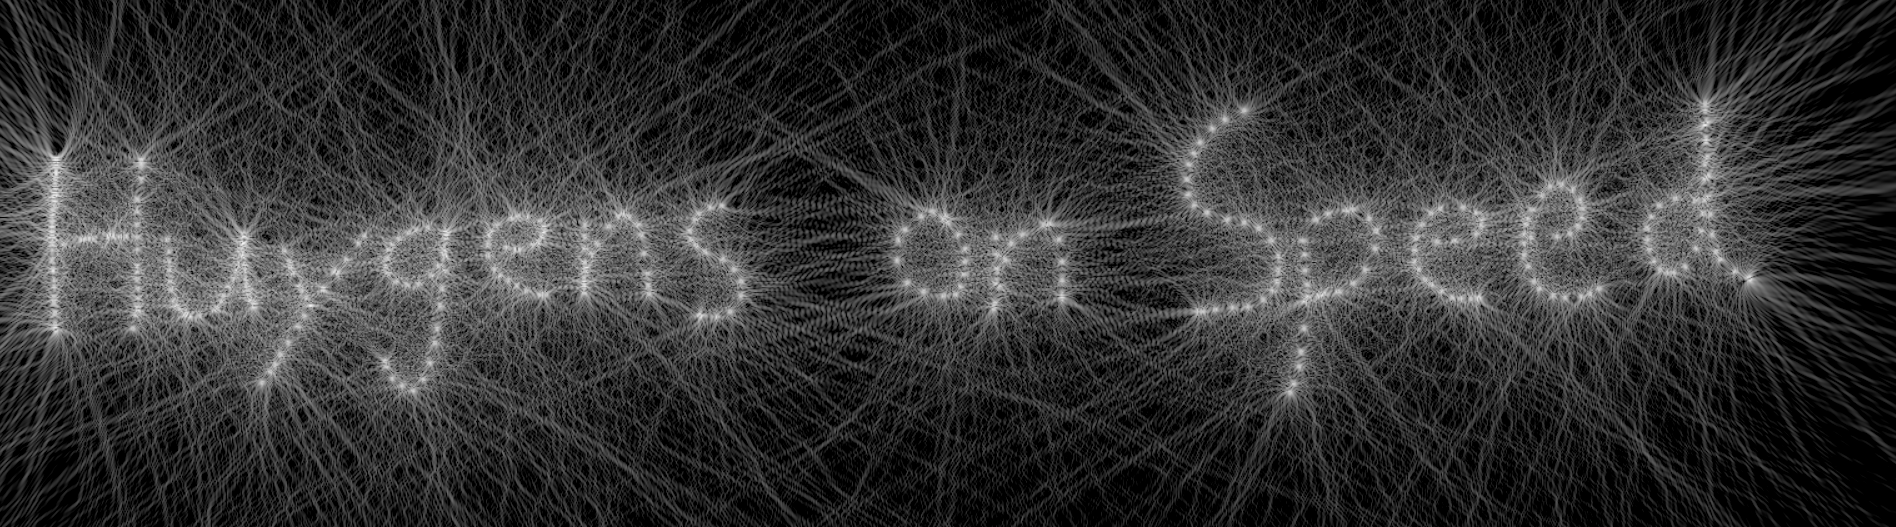
\includegraphics[width=\textwidth]{img/freeHandDrawing2.png}
\caption{Free hand drawing of source points using the interactive user interface.}
\label{fig:huygens_free_hand}
\end{figure*}

Implementing Huygens' principle on the GPU results in a significant speedup, that again allows for interactive simulations of dense pressure fields from acoustical arrays. We show this in Fig. \ref{fig:huygens_vs_ultrasim} by presenting a benchmark made between HOS and Ultrasim. Note that execution times are reported in seconds for Ultrasim and milliseconds for HOS. Thus the average speedup is 400x in favour of HOS across the selected range of source points. 

Fig. \ref{fig:lateral_pressure} shows the in-focus (at 80mm) lateral pressure from a 2.5MHz, 64 element ($32\lambda$ wide and $10\lambda$ high, $5 \text{ azimuth} \times 20 \text{ elevation}$ points/subelements per aperture) uniform linear array calculated with HOS, Field II and Ultrasim. The beam profiles are strikingly similar. In Fig. \ref{fig:radial_pressure} we also see that all three simulators yield the same result along an axial cut through focus. The continuous pressure field calculated with Field II was found by taking the fourier transform of the total transmit beam energy at the center frequency. 
%Better element directivity might cause the focus offset using Field II compared with the other simulators.

Fig. \ref{fig:huygens_vs_ultrasim_pressure_field} shows the azimuth pressure field calculated using HOS (a) and Ultrasim (b). The resolution is 5.6 observation points per mm for both, hence 250K observation points in total. HOS and Ultrasim used 2 seconds and 3 minutes 40 seconds respectively in order to generate the image, hence a 110x speedup. The hardware used in this comparison was an Nvidia GT520, 48 cores GPU, and a i7-870 Intel quad-core CPU. A multi threaded C-version of the presented simulator used 1 minute and 45 seconds to generate the same image. Field II used 2 minutes 51 seconds. Note that Field II has to calculate the spatial impulse response for all observation points, and is therefore not directly comparable to Ultrasim's snap-shot-mode. The spatial impulse response can be calculated using HOS by iterating in time. Using the available low-end GPU and high-end CPU, the presented simulator and Field II are equally fast on this operation (without using streams on the GPU). However, for massive parallel calculation of the spatial impulse response one might want to apply a different parallelization scheme and level of granularity than what is described in this paper.

Fig. \ref{fig:huygens_free_hand} shows how arrays of any shape can be interactively drawn using the provided user interface. A video of how the interactive user interface works can be found at \cite{hos}.

% An example of a floating figure using the graphicx package.
% Note that \label must occur AFTER (or within) \caption.
% For figures, \caption should occur after the \includegraphics.
% Note that IEEEtran v1.7 and later has special internal code that
% is designed to preserve the operation of \label within \caption
% even when the captionsoff option is in effect. However, because
% of issues like this, it may be the safest practice to put all your
% \label just after \caption rather than within \caption{}.
%
% Reminder: the "draftcls" or "draftclsnofoot", not "draft", class
% option should be used if it is desired that the figures are to be
% displayed while in draft mode.
%
%\begin{figure}[!t]
%\centering
%\includegraphics[width=2.5in]{myfigure}
% where an .eps filename suffix will be assumed under latex, 
% and a .pdf suffix will be assumed for pdflatex; or what has been declared
% via \DeclareGraphicsExtensions.
%\caption{Simulation Results}
%\label{fig_sim}
%\end{figure}

% Note that IEEE typically puts floats only at the top, even when this
% results in a large percentage of a column being occupied by floats.


% An example of a double column floating figure using two subfigures.
% (The subfig.sty package must be loaded for this to work.)
% The subfigure \label commands are set within each subfloat command, the
% \label for the overall figure must come after \caption.
% \hfil must be used as a separator to get equal spacing.
% The subfigure.sty package works much the same way, except \subfigure is
% used instead of \subfloat.
%
%\begin{figure*}[!t]
%\centerline{\subfloat[Case I]\includegraphics[width=2.5in]{subfigcase1}%
%\label{fig_first_case}}
%\hfil
%\subfloat[Case II]{\includegraphics[width=2.5in]{subfigcase2}%
%\label{fig_second_case}}}
%\caption{Simulation results}
%\label{fig_sim}
%\end{figure*}
%
% Note that often IEEE papers with subfigures do not employ subfigure
% captions (using the optional argument to \subfloat), but instead will
% reference/describe all of them (a), (b), etc., within the main caption.


% An example of a floating table. Note that, for IEEE style tables, the 
% \caption command should come BEFORE the table. Table text will default to
% \footnotesize as IEEE normally uses this smaller font for tables.
% The \label must come after \caption as always.
%
%\begin{table}[!t]
%% increase table row spacing, adjust to taste
%\renewcommand{\arraystretch}{1.3}
% if using array.sty, it might be a good idea to tweak the value of
% \extrarowheight as needed to properly center the text within the cells
%\caption{An Example of a Table}
%\label{table_example}
%\centering
%% Some packages, such as MDW tools, offer better commands for making tables
%% than the plain LaTeX2e tabular which is used here.
%\begin{tabular}{|c||c|}
%\hline
%One & Two\\
%\hline
%Three & Four\\
%\hline
%\end{tabular}
%\end{table}


% Note that IEEE does not put floats in the very first column - or typically
% anywhere on the first page for that matter. Also, in-text middle ("here")
% positioning is not used. Most IEEE journals/conferences use top floats
% exclusively. Note that, LaTeX2e, unlike IEEE journals/conferences, places
% footnotes above bottom floats. This can be corrected via the \fnbelowfloat
% command of the stfloats package.



%\section{Conclusion}
%The conclusion goes here.




% conference papers do not normally have an appendix

The simulator can be downloaded from the same site \cite{hos}. The source code has been made available at github \cite{hosGit}. Contributions are welcome.

% use section* for acknowledgement
\section*{Acknowledgment}
The authors would like to thank Tore Bj\aa{}stad, Torbj\o{}rn Hergum and Hans Torp for the initial idea of creating the HOS simulator.


